\documentclass[UTF8]{ctexart}
\usepackage{fancyhdr}
\usepackage{graphicx}
\usepackage{titlesec}
\usepackage{titletoc}
\usepackage{listings}
\usepackage{appendix}
\usepackage{bm, amsmath,amsfonts}
\usepackage{multirow}
\usepackage[a4paper,left=3.4cm,right=3cm,top=1.65cm,bottom=2.54cm]{geometry}
\usepackage{float}

\numberwithin{figure}{section}
\graphicspath{{figures/}}%定义图片存放的路径


\renewcommand{\contentsname}{\zihao{3} 目\quad 录}
\renewcommand{\abstractname}{\zihao{3} 摘\quad 要}
%页眉页脚设置
\pagestyle{fancy}
\fancyhf{}
\cfoot{\thepage}
\rhead{\kaishu~《XX》课程设计~} %这里是页眉

%目录页设置
\titlecontents{section}[0em]{\zihao{4}\bf }{\thecontentslabel\ }{}
{\hspace{.5em}\titlerule*[4pt]{$\cdot$}\contentspage}
\titlecontents{subsection}[2em]{\vspace{0.1\baselineskip}\zihao{-4}}{\thecontentslabel\ }{}
{\hspace{.5em}\titlerule*[4pt]{$\cdot$}\contentspage}
\titlecontents{subsubsection}[4em]{\vspace{0.1\baselineskip}\zihao{-4}}{\thecontentslabel\ }{}
{\hspace{.5em}\titlerule*[4pt]{$\cdot$}\contentspage}
%代码设置
\RequirePackage{listings}
\RequirePackage{xcolor}
\definecolor{dkgreen}{rgb}{0,0.6,0}
\definecolor{gray}{rgb}{0.5,0.5,0.5}
\definecolor{mauve}{rgb}{0.58,0,0.82}
\lstset{
	numbers=left,  
	frame=tb,
	aboveskip=3mm,
	belowskip=3mm,
	showstringspaces=false,
	columns=flexible,
	framerule=1pt,
	rulecolor=\color{gray!35},
	backgroundcolor=\color{gray!5},
	basicstyle={\ttfamily},
	numberstyle=\tiny\color{gray},
	keywordstyle=\color{blue},
	commentstyle=\color{dkgreen},
	stringstyle=\color{mauve},
	breaklines=true,
	breakatwhitespace=true,
	tabsize=3,
}
%------------------------------------------------------------------------
%正文部分
\begin{document}
\begin{titlepage}
	\centering
	\vspace*{1.75cm}
	\quad
\includegraphics[width= .9\textwidth]{AHUT_Logo.png}\\
	\vspace*{2cm}
	{\fontsize{20pt}\baselineskip 《JAVA程序设计》课程设计}
	\vskip 0.5cm
		{\fontsize{20pt}\baselineskip 实验报告书}
	\vskip 6cm
	\fontsize{19pt}\baselineskip
	\makebox[30mm]{设计题目}
	\underline{\makebox[75mm][c]{ XXXXXX}}\\%在这里修改成自己的题目
	\vskip 0.9cm
	\makebox[30mm]{学生姓名}
	\underline{\makebox[75mm][c]{ XX}}\\
	\vskip 0.9cm
	\makebox[30mm]{学\qquad\qquad 号}
	\underline{\makebox[75mm][c]{ \LARGE 199XXXXXX}}\\
	\vskip 0.9cm
	\makebox[30mm]{专业班级}
	\underline{\makebox[75mm][c]{ \LARGE XXX}}\\
	\vskip 0.9cm
	\makebox[30mm]{指导教师}
	\underline{\makebox[75mm][c]{ XXX}}\\
	\vskip 2cm
	\centerline{\large{计算机科学与技术学院}}
	\vskip 0cm
	\LARGE \textbf{\number \year }~年~\textbf{\number\month}~月~\textbf{\number\day}~日
\end{titlepage}

\begin{abstract}
	\pagestyle{plain}
	\thispagestyle{empty}
	\zihao{-4}
	视频提供了功能强大的方法帮助您证明您的观点。当您单击联机视频时,可以在想要添加的视频的嵌入代码中进行粘贴。您也可以键入一个关键字以联机搜索最适合您的文档的视频。为使您的文档具有专业外观,Word 提供了页眉、页脚、封面和文本框设计,这些设计可互为补充。例如,您可以添加匹配的封面、页眉和提要栏。单击“插入”,然后从不同库中选择所需元素。
	\par 主题和样式也有助于文档保持协调。当您单击设计并选择新的主题时,图片、图表或 SmartArt 图形将会更改以匹配新的主题。当应用样式时,您的标题会进行更改以匹配新的主题。使用在需要位置出现的新按钮在 Word 中保存时间。若要更改图片适应文档的方式,请单击该图片,图片旁边将会显示布局选项按钮。当处理表格时,单击要添加行或列的位置,然后单击加号。


	\textbf{关键字}:\quad 关键字 \quad 关键字 \quad 关键字 \quad 关键字
	\newpage
\end{abstract}

\tableofcontents\thispagestyle{empty}
\newpage
\setcounter{page}{1}
\section{文字排版}
\subsection{插入文字}
在新的阅读视图中阅读更加容易。可以折叠文档某些部分并关注所需文本。如果在达到结尾处之前需要停止读取,Word 会记住您的停止位置 - 即使在另一个设备上。视频提供了功能强大的方法帮助您证明您的观点。当您单击联机视频时,可以在想要添加的视频的嵌入代码中进行粘贴。您也可以键入一个关键字以联机搜索最适合您的文档的视频。
\par 为使您的文档具有专业外观,Word 提供了页眉、页脚、封面和文本框设计,这些设计可互为补充。例如,您可以添加匹配的封面、页眉和提要栏。单击“插入”,然后从不同库中选择所需元素。主题和样式也有助于文档保持协调。当您单击设计并选择新的主题时,图片、图表或 SmartArt 图形将会更改以匹配新的主题。当应用样式时,您的标题会进行更改以匹配新的主题。


\subsection{列出清单}
\par 本系统实现以下功能模块:
\begin{itemize}
	\item[1)] 功能1
	\item[2)] 功能2
	\item[3)] 功能3
\end{itemize}
\section{公式排版}
\subsection{插入公式}
\[
	3/8 \qquad \frac{3}{8}
	\qquad \tfrac{3}{8}
\]

\[
	a^2  = b^2 + c^2
\]

\section{图片排版}
\subsection{插入图片}
\subsubsection{单栏插入}

\begin{figure}[H]
	\centering
	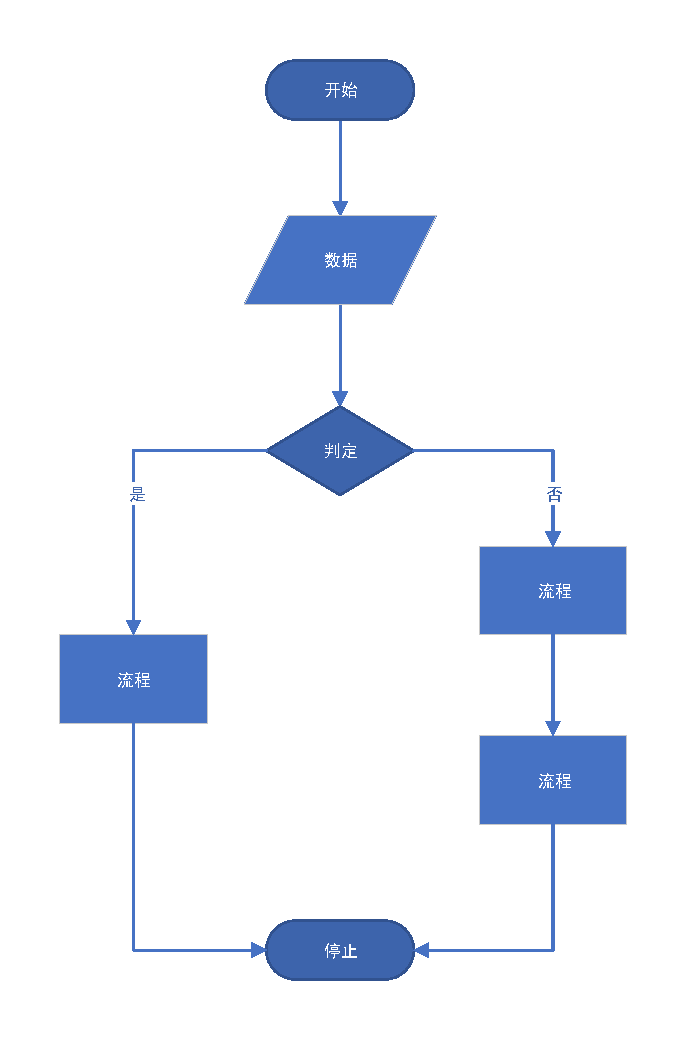
\includegraphics [width=0.6\textwidth]{测试.pdf}
	\caption{测试}
\end{figure}



\subsubsection{双栏插入}


\begin{figure}[H]
	\centering
	\begin{minipage}[c]{0.5\textwidth}
		\centering
		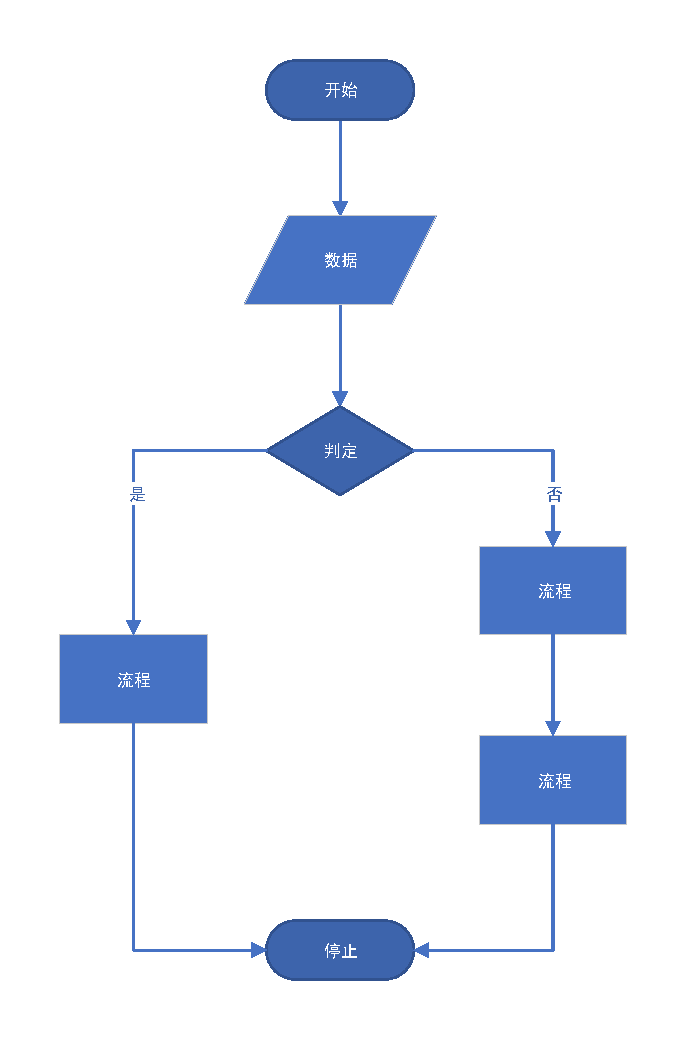
\includegraphics[width=1\textwidth]{测试.pdf}
		\caption{测试}
	\end{minipage}%
	\begin{minipage}[c]{0.5\textwidth}
		\centering
		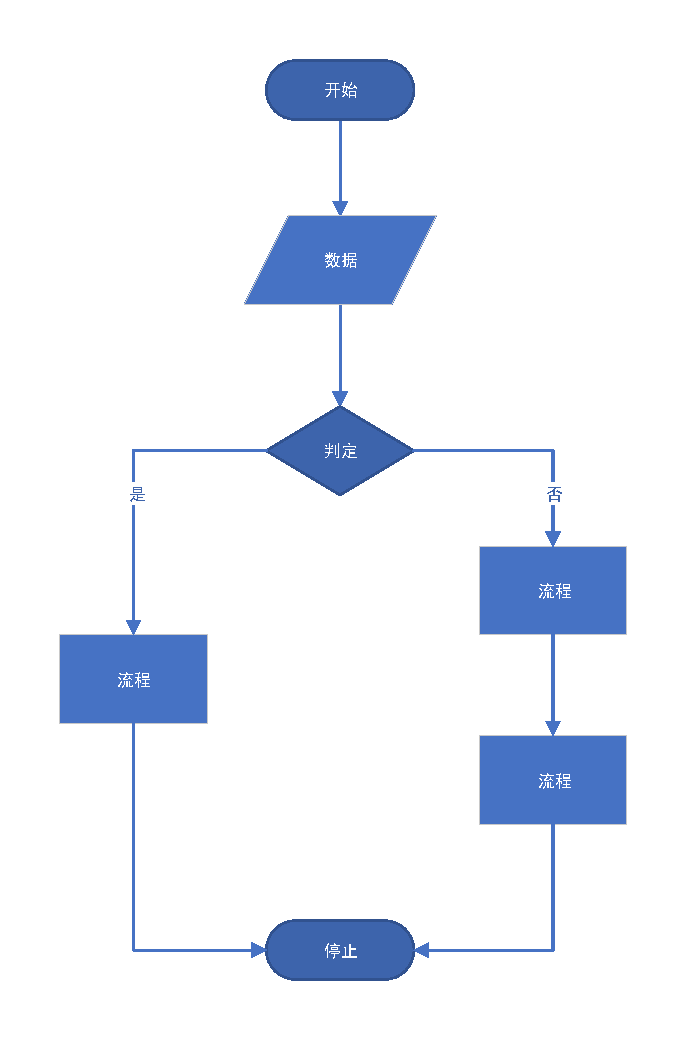
\includegraphics[width=1\textwidth]{测试.pdf}
		\caption{测试.pdf}
	\end{minipage}
\end{figure}


\section{代码排版}
\subsection{SQL语句}

\begin{lstlisting}[language=SQL,escapeinside=``]
--------------------------------------------------------
--  DDL for Table T_STUDENT
--------------------------------------------------------

  CREATE TABLE "XX" 
   (	"XX" VARCHAR2(20 BYTE), 
	"XX1" VARCHAR2(20 BYTE), 
	"XX2" VARCHAR2(20 BYTE), 
	"XX3" VARCHAR2(20 BYTE), 
	"XX4" VARCHAR2(20 BYTE), 
	"XX5" VARCHAR2(20 BYTE), 
	"XX6" VARCHAR2(20 BYTE)
   );
--------------------------------------------------------
--  Constraints for Table T_STUDENT
--------------------------------------------------------

  ALTER TABLE "XX" ADD CONSTRAINT "T_STUDENT_PK" PRIMARY KEY ("XX1");
  ALTER TABLE "XX" MODIFY ("XX1" NOT NULL ENABLE);
  ALTER TABLE "SXX" MODIFY ("XX2" NOT NULL ENABLE);

\end{lstlisting}


\subsection{C语言}
\begin{lstlisting}[language=C,escapeinside=``]
#include<stdio.h)
int main() {
	printf("Hello World");
	return 0;
}
\end{lstlisting}
\subsection{JAVA}
\begin{lstlisting}[language=JAVA,escapeinside=``]
	public class HelloWorld {
		public static void main(String[] args){
			System.out.println("Hello World");
		}
	}
	
\end{lstlisting}



\newpage
\section{总结}

\newpage
\begin{appendices}
	\section{系统说明}

	\subsection{开发环境}

	\subsection{系统部署}

\end{appendices}

\end{document}